\subsection{Nao Hardware}
The Nao Humanoid Platform is made by Aldebaran Robotics. 
Figure~\ref{fig:crrl_nao_coronal1} shows a picture of the Nao at the
Control/Robotics Research Lab of NYU Polytechnic School of Engineering.
The robot weighs $5.4 kg$ and has a maximum forward velocity over flat
terrain of approximately $1 \frac{m}{s}$.
It has 25 degrees-of-freedom (DoF) embodied via a 2 DoF head, two 5 DoF legs,
two 5 DoF arms, two 1 DoF hands, and a 1 DoF hip.
Figure~\ref{fig:nao_joints1} shows a diagram locating each of the joints on
the robot.
% Sonars, joint sensors, cameras, foot sensors, IMU, bumpers and buttons.
Each joint has an absolute angular position encoder, while the feet each have
four force sensitive resistors to detect ground contact.
The head has two color cameras, one that faces forward and the other that faces
downward to get a view of the terrain. The chest contains a 2-axis gyroscope and
a 3-axis accelerometer for inertial measurement, and two sonar transmitter-receiver
pairs for measuring the range to obstacles.
Figure~\ref{fig:nao_features1} shows a diagram locating the various robot sensors,
including those not listed above.
% Battery life, weight, top speed (before and after Lidar), sonar ranges, camera angles and pixels,
The sonars have a minimum range of $0.25 m$ and a maximum range of $2.55 m$.
They have a resolution of $1 cm$ and detect any obstacle within a $60^\circ$
cone. The cameras have a $1.22 Mp$ resolution, $30 Hz$ frame rate,
a horizontal field-of-view of $60.9^\circ$, and a vertical field-of-view of
$47.6^\circ$.
% CPU type and speed, RAM, storage space, USB, Ethernet, WiFi.
The robot is equipped with a 1.6 GHz Intel\textsuperscript{\textregistered}
Atom\textsuperscript{TM} CPU, 1 GB of RAM, and 2 GB of Flash memory.
It also has Gigabit Ethernet, 802.11 b/g/n WiFi, and USB 2.0. 
Nao's operating system is called NAOqi OS which is a customized version of
Gentoo Linux. Being a Linux distribution, the robot can be easily accessed
using ssh, scp, and ftp. This allows familiar command line tools to be used
to script behavior and manage services.
The robot can be natively programmed using the provided C++ or Python API.

% Ok, now briefly review what's to come in the subsubsections.
The Nao is a very feature rich platform suitable for a variety of autonomous
applications. The following sections will review specific aspects of the robot
relevant to Chapters~\ref{ch:results_navigation} and~\ref{ch:results_crawling}.


\begin{figure}
\centering
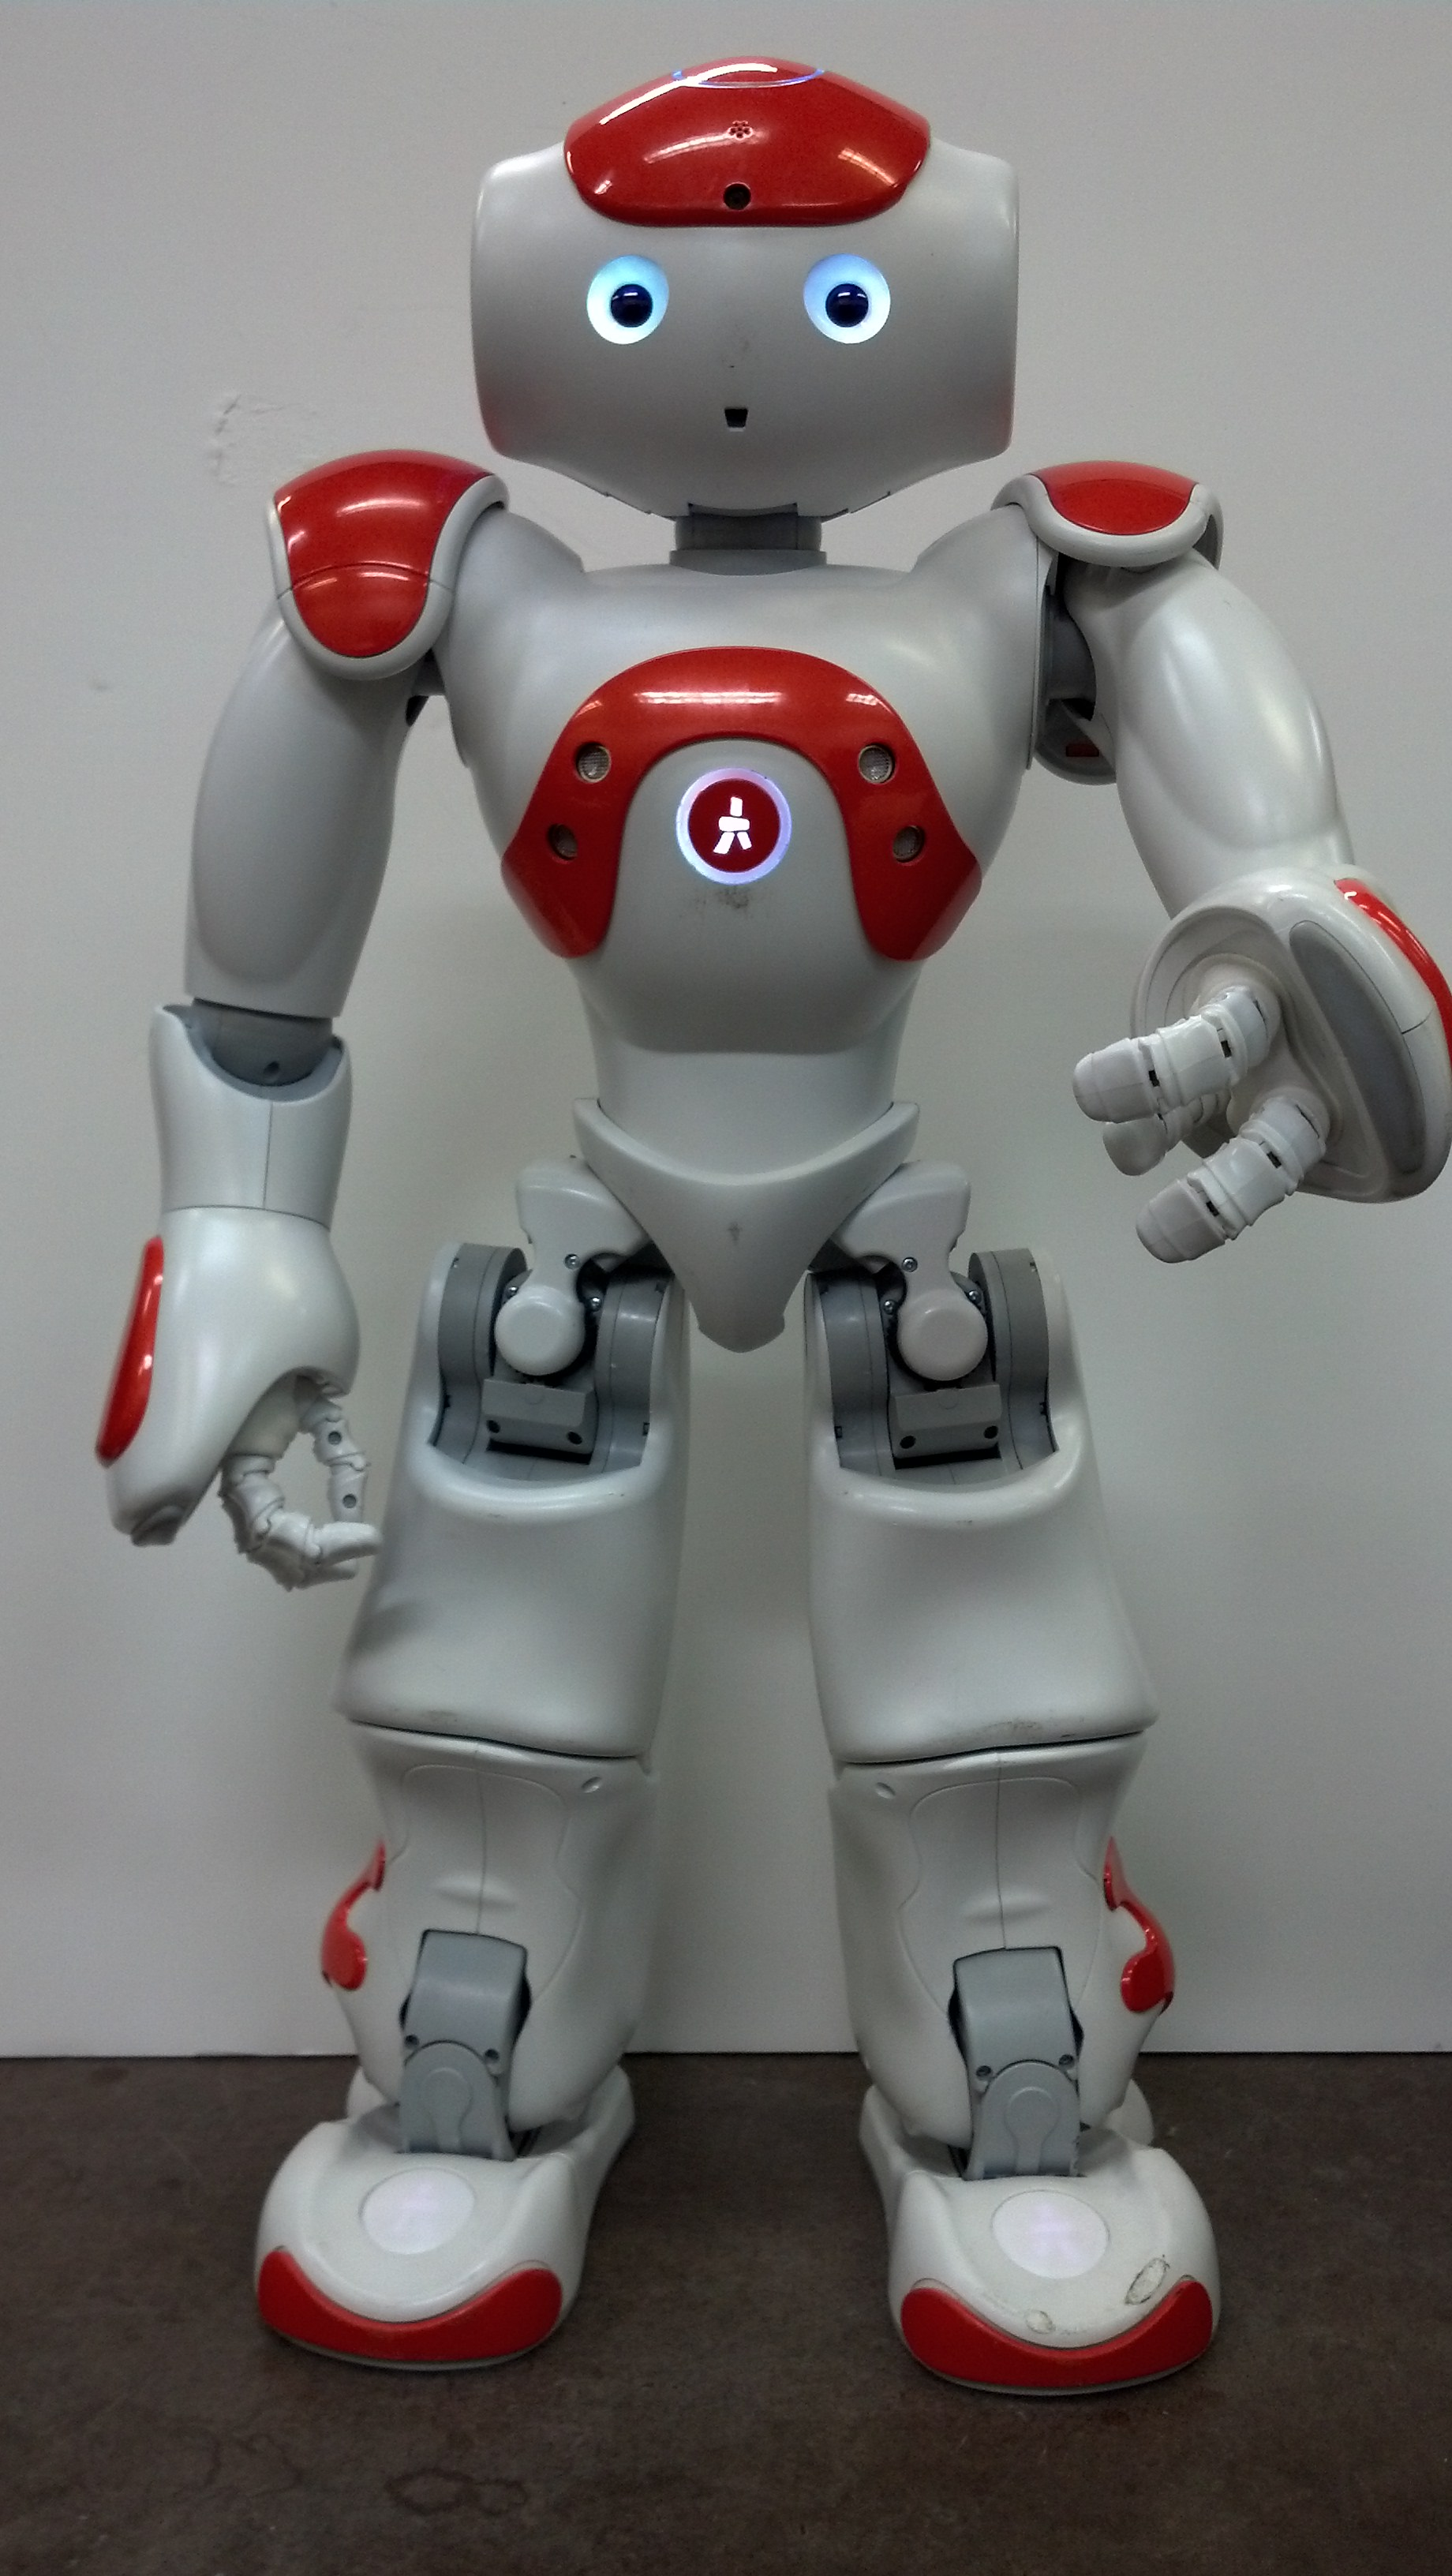
\includegraphics[height=0.4\textheight]{nao_coronal1.jpg}
\caption{Figure showing the Nao Humanoid Platform at the Control/Robotics
         Research Lab at NYU Polytechnic School of Engineering.}
\label{fig:crrl_nao_coronal1}
\end{figure}

\begin{figure}
\centering
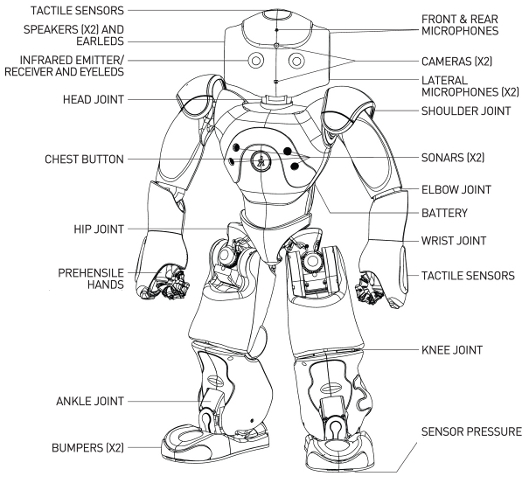
\includegraphics[width=0.4\textheight]{nao_diagrams/nao_h25_pres.png}
\caption{Figure locating the various features on the robot.}
\label{fig:nao_features1}
\end{figure}

\begin{figure}
\centering
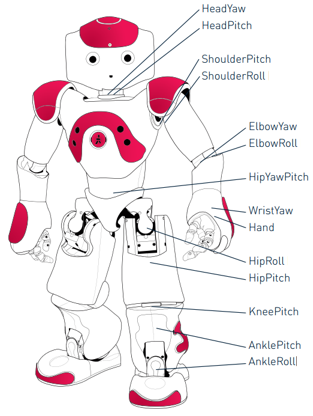
\includegraphics[height=0.4\textheight]{nao_diagrams/hardware_motortype_h25V5.png}
\caption{Figure indicating the various joint locations and their names.}
\label{fig:nao_joints1}
\end{figure}

\FloatBarrier

\subsubsection{Frame Definitions}
The NAOqi API defines three frames that can be seen in Figure~\ref{fig:nao_frames1}.
They are FRAME\_TORSO, FRAME\_ROBOT, and FRAME\_WORLD\@.
The first two frames, FRAME\_TORSO and FRAME\_ROBOT, are rigidly
attached to the robot, while FRAME\_WORLD is an inertial frame initialized
when the robot first starts.

\paragraph{FRAME\_TORSO} 
is a frame rigidly attached to the torso of the Nao. The positive Z-axis points
up through the head of the robot, while the positive X-axis points forwards.
It is useful for referencing different parts of the robot such and joint frames
and manipulation targets relative to the robot.
The frame origin along the X and Y directions is in the geometric center
of the torso, while Figure~\ref{fig:nao_link_lengths1} shows its Z location on
the torso as the point that the neck and hip offsets are referenced with
respect to.

\paragraph{FRAME\_ROBOT}
is a frame whose origin is between the feet of the robot. It's positive Z-axis
always points upwards and positive X-axis always points forwards. It is useful
when specifying navigation targets, relative to the Nao's current pose.

\paragraph{FRAME\_WORLD}
is a frame that is coincident with FRAME\_ROBOT when the Nao is started,
and remains static for the life of the run. It is useful for specifying navigation
and manipulation targets in a global coordinate sense.

\begin{figure}[H]
\centering
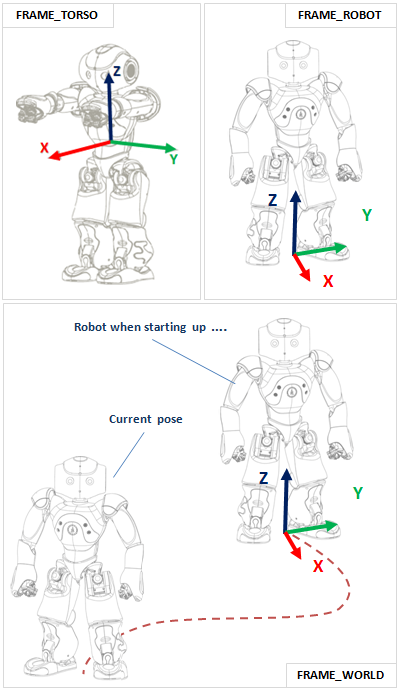
\includegraphics[height=0.75\textheight]{nao_diagrams/frame_definition_combo.png}
\caption{Nao frames.}
\label{fig:nao_frames1}
\end{figure}

Orientation targets for the Nao are commonly expressed using Tait-Bryan angles,
more commonly known as roll, pitch, and yaw. As can be seen in
Figure~\ref{fig:nao_rpy_def1}, yaw is expressed as rotation about the Z-axis,
roll is about the X-axis, and pitch is about the Y-axis.
When the robot is being referenced from the FRAME\_TORSO and is
initialized in the StandZero posture referenced in the proceeding section,
the naming conventions of the joints become clear. All joints whose axis
are parallel to the torso frame Y-axis are postfixed with the word ``Pitch'',
those parallel to the Z-axis are postfixed with the word ``Yaw'', and X-axis
with ``Roll''. The only exception to this rule is the ganged pelvis joint
axis. Each side of this degree of freedom rotates along a vector that is
in the plane formed by the torso Z-Y axes and is therefore postfixed with the
term ``YawPitch''.

\begin{figure}
\centerline{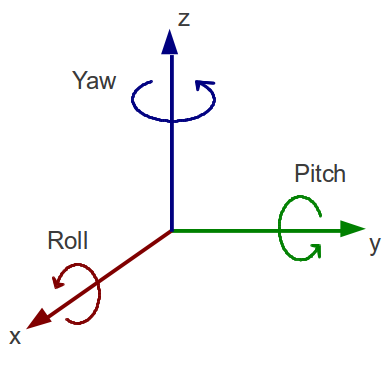
\includegraphics[width=0.5\textwidth]{nao_diagrams/rollPitchYaw.png}
}
\caption{Definition of roll pitch and yaw.}
\label{fig:nao_rpy_def1}
\end{figure}


\subsubsection{Links and Joints}
The Nao H25 is a bipedal platform with two legs, two arms, and an articulate
head. Each arm is composed of 5 joints and 3 non-zero length links, as are 
the legs, and the head is composed of 2 joints. There are also three fingers
per hand and two feet. Detailed measurements and specifications on the
Nao H25 can be found on the Aldebaran Website~\cite{nao_docs_h25}.
We will review a few relevant characteristics of the robot below.

\paragraph{Links}
Figure~\ref{fig:nao_link_lengths1} shows some of the large scale link lengths
of the Nao H25. The hip and neck Z offsets are measured with respect to
FRAME\_TORSO, as are the shoulder and hip Y offsets. The thigh and tibia lengths
are each roughly $100 mm$. Their total is $202.8 mm$. The neck and hip offsets
sum to $211.5$, making the torso approximately the same length as the legs.
The humerus of the robot is again nearly $100 mm$ though the forearm to the wrist
is half as long. The wrist to the hand is again about half as long as the
humerus, meaning in total, the arms are about as long and the legs.

\begin{figure}
\centerline{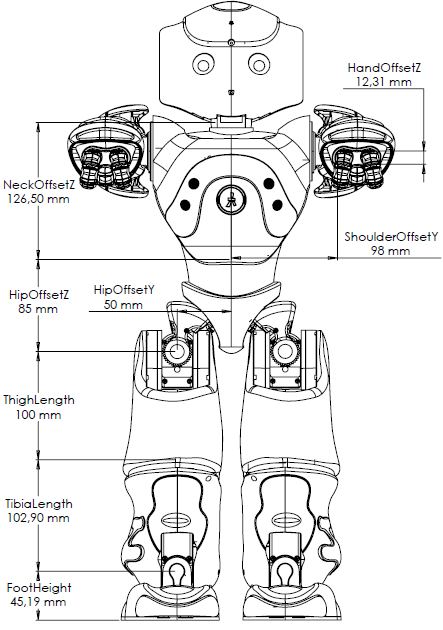
\includegraphics[width=0.45\textwidth]{nao_diagrams/hardware_lengthfront_3.3.png}
            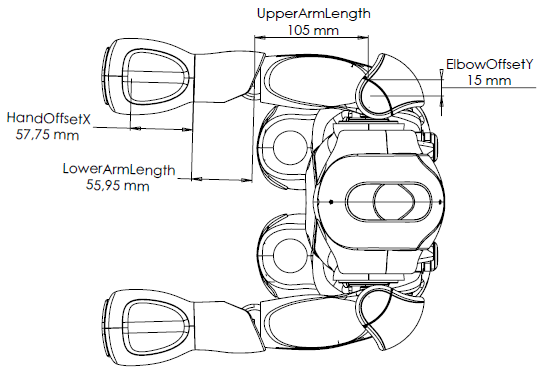
\includegraphics[width=0.55\textwidth]{nao_diagrams/hardware_lengthup_3.3.png}
}
\caption{Nao link lengths.}
\label{fig:nao_link_lengths1}
\end{figure}

\paragraph{Joints}
This needs to be said.
In the below diagrams, the green line represents the nominal zero, the blue line
is the min angle, and the red line is the max angle
\begin{figure}
\centering
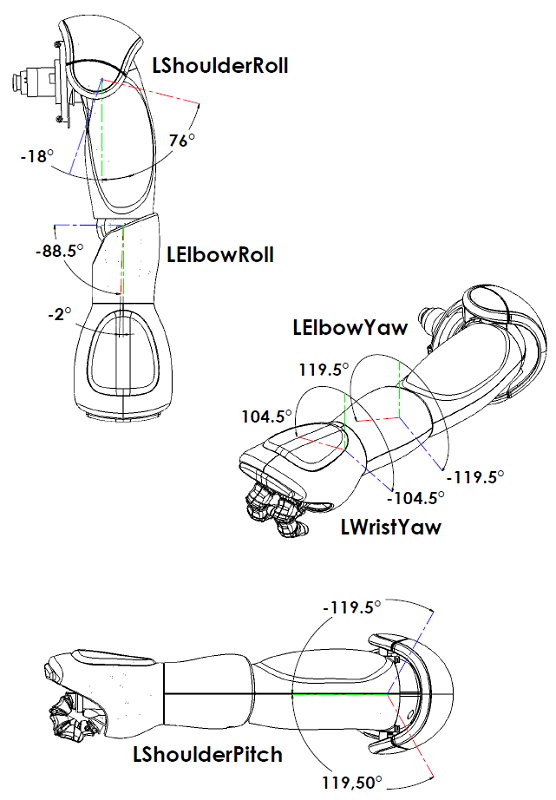
\includegraphics[width=\textwidth]{nao_diagrams/hardware_larmjoint_3.3_corr1.png}
\caption{Figure showing left arm}
\label{fig:nao_arm_joints_left1}
\end{figure}

\begin{figure}
\centering
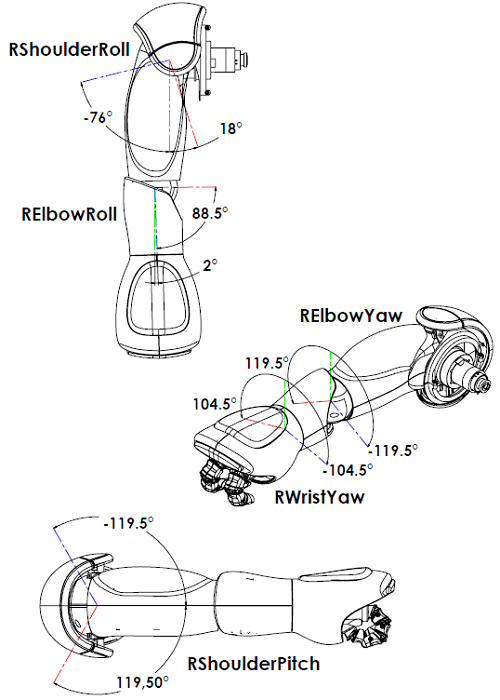
\includegraphics[width=\textwidth]{nao_diagrams/hardware_rarmjoint_3.3.png}
\caption{Figure showing right arm}
\label{fig:nao_arm_joints_right1}
\end{figure}

\begin{figure}
\centering
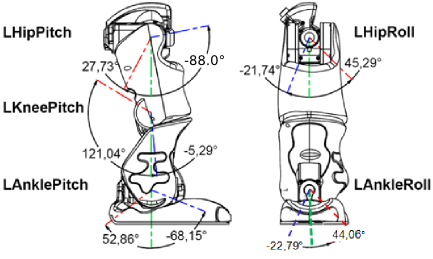
\includegraphics[width=\textwidth]{nao_diagrams/hardware_llegjoint.png}
\caption{Figure showing left leg}
\label{fig:nao_leg_joints_left1}
\end{figure}

\begin{figure}
\centering
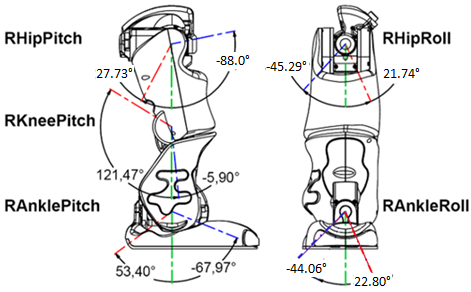
\includegraphics[width=\textwidth]{nao_diagrams/hardware_rlegjoint.png}
\caption{Figure showing right leg}
\label{fig:nao_leg_joints_right1}
\end{figure}

\begin{figure}
\centering
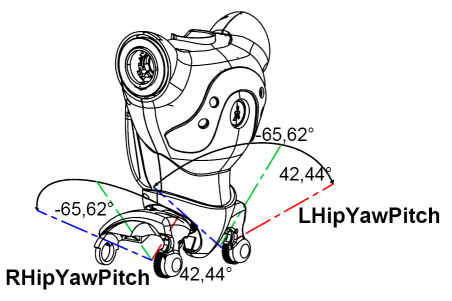
\includegraphics[width=\textwidth]{nao_diagrams/hardware_pelvisjoint.png}
\caption{Figure showing hip yaw-pitch}
\label{fig:nao_hip_yawpitch1}
\end{figure}

\paragraph{Arm Symmetry}
Need diagram showing arm symmetry for crawl results. 

\begin{figure}
\centering
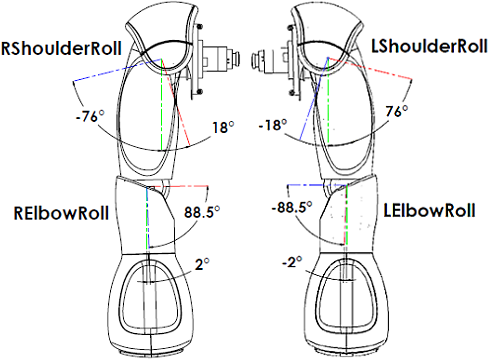
\includegraphics[width=\textwidth]{hardware_r_and_l_armjoint_corr1.png}
\caption{Figure showing arm joints and how they are a reflection.}
\label{fig:nao_arm_joints_reflect1}
\end{figure}

\FloatBarrier

\subsubsection{Joint Torques}
% Motor torques. (Important for Chapter~\ref{ch:crawl_gait})
Talking about the joint motor torques, tables, gearboxes, blah.

\subsubsection{Postures}
Talking about the different postures of the robot.

\begin{figure}
\centerline{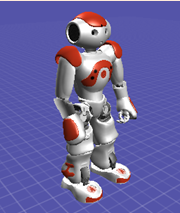
\includegraphics[width=0.33\textwidth]{posture/posture_stand.png}
            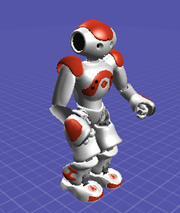
\includegraphics[width=0.33\textwidth]{posture/posture_standinit.png}
            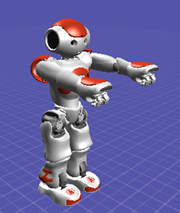
\includegraphics[width=0.33\textwidth]{posture/posture_standzero.png}
}
\vspace*{0.05in}
\centerline{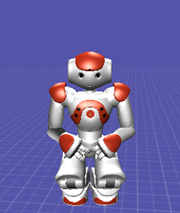
\includegraphics[width=0.33\textwidth]{posture/posture_crouch.png}
            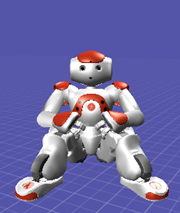
\includegraphics[width=0.33\textwidth]{posture/posture_sit.png}
            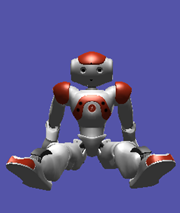
\includegraphics[width=0.33\textwidth]{posture/posture_sitrelax.png}
}
\vspace*{0.05in}
\centerline{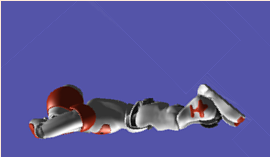
\includegraphics[width=0.5\textwidth]{posture/posture_lyingbelly.png}
            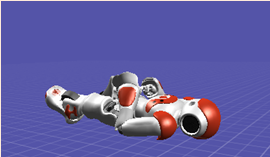
\includegraphics[width=0.5\textwidth]{posture/posture_lyingback.png}
}
\caption{Figure showing postures.}
\label{fig:nao_postures1}
\end{figure}
